%
% File acl2021.tex
%
%% Based on the style files for EMNLP 2020, which were
%% Based on the style files for ACL 2020, which were
%% Based on the style files for ACL 2018, NAACL 2018/19, which were
%% Based on the style files for ACL-2015, with some improvements
%%  taken from the NAACL-2016 style
%% Based on the style files for ACL-2014, which were, in turn,
%% based on ACL-2013, ACL-2012, ACL-2011, ACL-2010, ACL-IJCNLP-2009,
%% EACL-2009, IJCNLP-2008...
%% Based on the style files for EACL 2006 by 
%%e.agirre@ehu.es or Sergi.Balari@uab.es
%% and that of ACL 08 by Joakim Nivre and Noah Smith

\documentclass[11pt,a4paper]{article}
\usepackage[hyperref]{acl2021}
\usepackage{times}
\usepackage{latexsym}
\renewcommand{\UrlFont}{\ttfamily\small}

% This is not strictly necessary, and may be commented out,
% but it will improve the layout of the manuscript,
% and will typically save some space.
\usepackage{microtype}
\usepackage{inconsolata}
\usepackage{graphicx}
\usepackage{subfigure}
\usepackage{booktabs}
\usepackage{multirow}
\usepackage{makecell}
\usepackage{amsmath}
\usepackage{amssymb}
\usepackage{enumitem}

\aclfinalcopy % Uncomment this line for the final submission
%\def\aclpaperid{***} %  Enter the acl Paper ID here

%\setlength\titlebox{5cm}
% You can expand the titlebox if you need extra space
% to show all the authors. Please do not make the titlebox
% smaller than 5cm (the original size); we will check this
% in the camera-ready version and ask you to change it back.

\newcommand\BibTeX{B\textsc{ib}\TeX}

\title{Learning to Refer: How Scene Complexity Affects Emergent Communication in Neural Agents}

\author{Dominik Künkele$^{1}$ \and Simon Dobnik$^{1,2}$ \\
        Department of Philosophy, Linguistics and Theory of Science$^{1}$ \\ 
        Centre for Linguistic Theory and Studies in Probability (CLASP)$^{2}$ \\
        University of Gothenburg, Sweden \\
        \texttt{contact@dominik-kuenkele.de} \and \texttt{simon.dobnik@gu.se}}

\date{2025-08-19}

\begin{document}
\maketitle
\begin{abstract}
  We explore how neural network-based agents learn to map continuous sensory input to discrete linguistic symbols through interactive language games.
  One agent describes objects in 3D scenes using invented vocabulary; the other interprets references based on attributes like shape, color, and size.
  Learning is guided by feedback from successful interactions.
  We extend the CLEVR dataset with more complex scenes to study how increased referential complexity impacts language acquisition and symbol grounding in artificial agents.
\end{abstract}

\section{Introduction and Background}
How do cognitive systems bridge the gap between rich, continuous sensory experiences and the sparse, discrete symbols used in communication?
While perception operates through continuous signals, linguistic communication relies on finite vocabularies that must ground meaning about the perceived world \citep{Regier1996,Roy2005,Cooper2023}.
This representational challenge, known as the symbol grounding problem \citep{Harnad1990}, becomes particularly acute in artificial systems where discrete symbols must acquire meaning through interaction rather than pre-programmed associations.

Referring expressions require systems to map visual attributes onto linguistic descriptions that uniquely identify target objects and thus can be used to study symbol grounding.
\citet{Dale1995} formalized this process through an incremental generation algorithm that constructs descriptions by systematically adding distinguishing properties in order of salience until achieving unique identification.
By this, referring expression only contain attributes that are necessary to discriminate the target from the surroundings.

Research in this area investigates how artificial agents can develop referential abilities through language games - interactive scenarios where communication protocols emerge from repeated coordination attempts \citep{Clark1996,Bartlett2005,Kirby2008,Steels2009,Kharitonov2019,Lazaridou2017}.
Modern implementations use deep neural networks as agents that exchange discrete messages to solve visual discrimination tasks, allowing systematic study of how symbol meaning emerges from interaction.

This paper examines emergent referential communication in neural agents tasked with identifying objects in 3D visual scenes.
Using a highly controlled extension of the CLEVR dataset \citep{Johnson2017a}, we are able to manipulate the bias the neural agents are able to use in the emergent communication.
We are able to vary the complexity of referential scenarios to understand the constraints governing successful symbol grounding.
Our work is a study of how increasing the complexity of the scene (and therefore the space of potential referential expressions to be learned) affects learning through interaction of particular configurations of neural networks.

\section{Dataset}
\begin{figure*}[!htbp]
  \centering
  \subfigure['CLEVR color', \emph{small brown cylinder}]{
    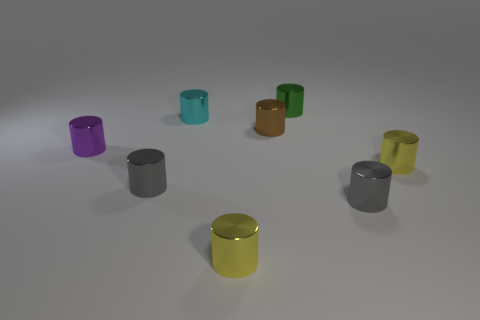
\includegraphics[width=0.3\linewidth]{figures/CLEVR_color.png}
    \label{fig:clevr-color}
  }
  \subfigure['Dale-2', \emph{small green cylinder}]{
    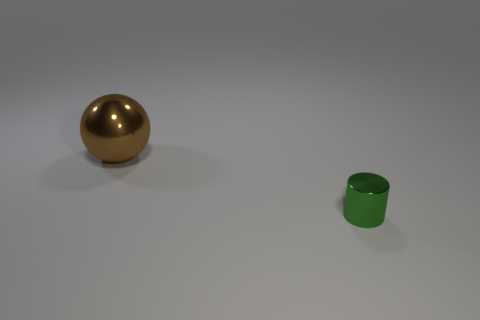
\includegraphics[width=0.3\linewidth]{figures/CLEVR_dale-2.png}
    \label{fig:clevr-dale-2}
  }
  \subfigure['Dale-5', \emph{large purple cylinder}]{
    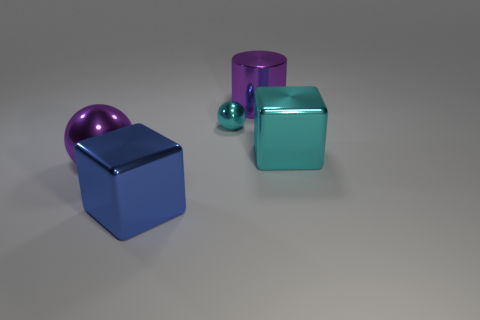
\includegraphics[width=0.3\linewidth]{figures/CLEVR_dale-5.png}
    \label{fig:clevr-dale-5}
  }
  \caption{Example images of each dataset, with the target object specified.}
  \label{fig:clevr-examples}
\end{figure*}

We extend the original CLEVR framework \citep{Johnson2017a} to have more control over the generated scenes.\footnote{\href{https://github.com/DominikKuenkele/MLT\_Master-Thesis\_clevr-dataset-gen}{github.com/DominikKuenkele/MLT\_Master-Thesis\_clevr-dataset-gen}}
By this, the objects in the generated images are controlled to have different human-recognizable attributes, namely the \emph{shape}, \emph{size} and \emph{color}.
These attributes also correspond to referring expressions in natural language such as English which effectively biases the agents to learn a language that is comparable to a human language.

The objects in the scene are separated into two categories: one \emph{target object} and a controlled number of \emph{distractor} objects.
The target object is the main object in the scene and the models are trained to identify and communicate it between each other.
This object is unique in the scene in respect to the attributes.
The distractor group contains objects that can share a maximum of two attributes per object.
Distractors are not required to be unique.

Using these rules, we generate three datasets with the following constraints:
(i) the size of the generated images is 480$\times$320 pixels;
(ii) 10.000 images are created for each of the datasets;
(iii) each image contains a maximum of 10 objects, that are not intersecting, have the same minimum distance between objects and are at least partially visible from the camera.

\subsection{CLEVR color}
The first generated dataset is called 'CLEVR color', in which the target object is identifiable by just the color.
Both \emph{shape} and \emph{size} of all distractors are shared with the target object.
The distractor group can contain in between 6 and 9 objects.

As seen in Figure \ref{fig:clevr-color}, the \emph{small brown cylinder} is unique.
By this, it is possible to refer to the target object using the attributes with four different combinations: the \emph{brown} object, the \emph{brown cylinder}, the \emph{small brown} object and the \emph{small brown cylinder}. % SD 2025-06-02 19:19:05 +0200: Just "the brown"?

\subsection{CLEVR Dale datasets}
The above described dataset is very restrictive in the relation between the objects, where only \emph{one} attribute is used to disambiguate them.
The number and the type of shared attributes are controlled exactly.
In the real world, objects have overlapping attributes and hence objects can often be identified by an intersection of multiple attributes.
For this, we created a dataset that allows almost any relation between a target object and the distractors.
The creation is inspired by the incremental algorithm for the Generation of Referring Expressions (GRE) described in \citep{Dale1995} who observe that attributes in descriptions occur in certain order and are added incrementally in a certain hierarchy.
This algorithm ensures that every scene contains a unique object in respect to its and the distractors' attributes.
Using the algorithm, one can refer to an object using its attributes to discriminate it from all other objects as efficiently as possible.
In other words, the object is described unambiguously using the lowest number of words.
On the other side, it is not controlled which attributes are shared; they are assigned randomly.

Two datasets following these rules are created.
The 'Dale-2' dataset contains one target object and one distractor (see Figure \ref{fig:clevr-dale-2}), while the Dale-5 dataset contains one target object and exactly four distractors.
Consider Figure \ref{fig:clevr-dale-5}, with the target object being the \emph{large purple cylinder}. The large purple sphere shares the size and color, the two cubes only share the size, and the small turquoise sphere doesn't share any attribute.

\section{Method}
\subsection{Image processing}
\label{sec:image-processing}
To extract the features and process the images of the datasets, we build upon the proposed architecture in \citet{Johnson2017} which was used to train baseline models on the original CLEVR dataset.
Hereby, the image is first passed through a frozen ResNet-101 model \citep{He2016}.
Two convolutional layers with subsequent \emph{ReLU} non-linearities condense the important information from the output of the feature extractor.
The convolutional layers reduce the channels to 128 channels, using a kernel size of 3 and a stride and padding of 1.
This matrix represents the encoded image with its extracted features.

\subsection{Language Games}
\label{sec:methodology:language-games}
The goal of this research is to run and compare different setups of language games systematically.
To do this, all experiments rely on the \emph{\textbf{E}mergence of lan\textbf{G}uage in \textbf{G}ames} (EGG) framework \citep{Kharitonov2019}.
This framework allows the implementation of language games in code, where two neural models agents communicate through a unidirectional discrete channel.
A sender agent processes visual input.
The result is used as the initial hidden state for the encoder LSTM.
This LSTM is then producing symbols until it generates an \texttt{<eos>} symbol.
The receivers' decoder LSTM processes the message symbol by symbol with a randomly initialized hidden state.
After each time, a symbol is processed by the LSTM, the resulting new hidden state is passed to the receiver's neural model as the parsed message.
The receiver agent is combining it with its representation of the image input and is predicting an output.
In other words the receiver agent produces as many outputs as symbols are present in the message.
The loss is calculated for each of these outputs separately.
These losses are summed up to a total loss that is used to adapt the weights in both agents as well as in both LSTMs.
As the discrete sampled categorical distribtion of the message can't be differentiated, we use Gumbel-Softmax relaxation \citep{Jang2017} to turn it into a continuous distribution, thus allowing backpropagation through the whole language game.

\section{Experiments}
\subsection{Attending in a language game}
\subsubsection*{Setup}
Two agents are tasked to solve a referring problem together.
The receiver needs to 'point' to the target object in the visual scene that the sender is describing.
However, only the sender is aware of which of the shown objects is the target object.
To solve the task correctly the sender is required to generate a referring expressions about the target object through the discrete channel while the receiver needs to resolve it.
The experiment is set up in a way that avoids explicit human language information as e.g. human referring expressions or one-hot encoded attributes.
Messages by the sender can only be based on the highly controlled implicit bias in the visual scenes.

\begin{figure}[ht]
  \centering
  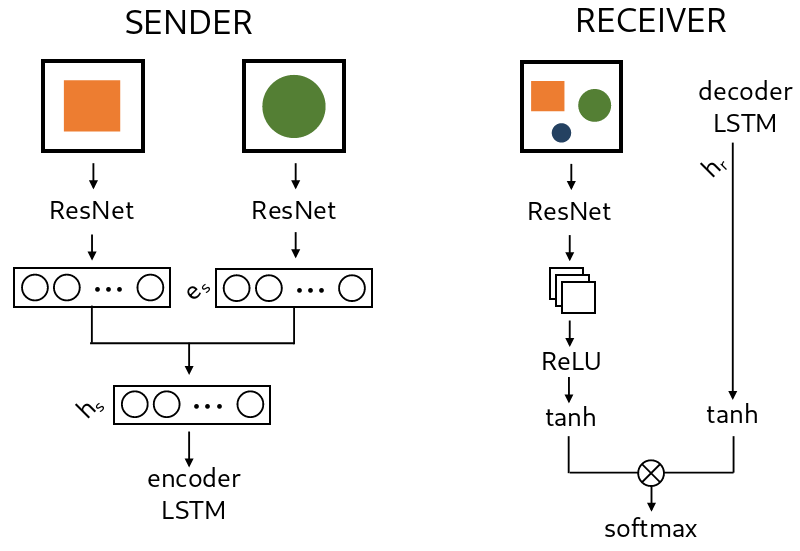
\includegraphics[width=\linewidth]{figures/arch_attention_predictor_game.png}
  \caption{Simplified architecture of the attention predictor game.}
  \label{fig:attention_predictor_game_architecture}
\end{figure}

Figure \ref{fig:attention_predictor_game_architecture} shows the simplified architecture of the language game.
The sender is given a set of bounding boxes of all objects in the scene, where the target object is always the first bounding box and the distractors are shuffled.
The features of each bounding box are extracted using ResNet-101, combined and passed to the LSTM to produce a message.
The receiver is shown the whole scene including the spatial information.
Given the sender's message, the task is to predict the region around target object.
For this, the image is divided into 14$\times$14 regions.
The target area is located around the center of the target object, consisting of 3$\times$3 regions.
The model is then tasked to predict the matrix $A = (a_{ij})$, where:
\begin{align*}
  a_{ij} =
  \begin{cases}
    1, & \text{if region $i,j$ in target area} \\
    0, & \text{otherwise}
  \end{cases}
\end{align*}

The image is encoded using a combination of ResNet-101 and several convolutional layers described in Section \ref{sec:image-processing}.
The resulting matrix has 128$\times$14$\times$14 dimensions, corresponding to the 14$\times$14 regions.

The sender's message is decoded using an LSTM and the dot product is calculated between each encoded region of the image and the encoded message.
The $softmax$ function is applied subsequently, which results in a 14$\times$14 matrix.
This emphasizes the correlation between the message and each region.
A high dot product for a region indicates a high correlation between the message and the specific region, while a low dot product indicates the opposite.
Training the agents like this should therefore highlight the regions in the image that are described by the sender, namely the region around the target object.
To calculate the loss, the $softmax$ function is applied over the prediction and compared to the ground truth matrix $A$ using \emph{binary cross entropy}.
More details can be found in Appendix \ref{app:technical-details-language-games}.
A total of 128.000 games are played.
Furthermore, we allow message lengths of $n \in \{1,2,3,4,6\}$ and provide vocabulary sizes of $|V| \in \{2,10,16,50,100\}$.

The agents are evaluated on the summed predicted probability for the regions in the target area, the probability mass.
In particular, the predicted matrix, consisting of probabilities for each region is multiplied with the ground truth matrix $A$, consisting of only ones and zeros.
The result is summed and returns the probability mass for the target area.
If the model predicts the target area perfectly, the probabilities in the target area sum to 1.
If the model for instance focuses on the wrong object, the probability mass in the target area is lower.

All results are compared to a baseline in which the sender is generating random messages, so that the receiver needs to solve the task on its own.
Any increase in performance requires information being transferred between the agents and the emergence of a language.

% SD 2025-06-02 19:34:52 +0200: Some of the technical details about the exact structure of the LSTMs and the parameters could be moved to Appendix (and referenced) to save space.
% DK 2025-06-03 10:00:00 +0200: (done)

\subsubsection*{Results}
The learning curves are shown in Figure \ref{fig:learning-curves_attention-predictor}.
As can be seen, the agents are able to solve the task across all datasets, but with different consistency.
However, when the agents start to learn to communicate, the probability mass is boosted instantly to a higher level, where it again learns at a slower speed parallel to the baseline.
On the 'Dale-2' dataset, the boost is around 40\% points.
Most of the learning takes place in the first 40.000 games, but there are also two configurations that increase the performance very late after 70.000 and 105.000 games respectively.
Hereby, agents tend to learn faster the smaller their vocabulary size is.
Using the 'Dale-5' dataset, the probability masses are boosted around 30\% points when the agents start to communicate successfully.
Compared to the 'Dale-2' dataset, fewer configurations start to converge, while most achieve performances close to the baseline. % SD 2025-06-02 19:48:52 +0200: What is the baseline?
The smaller number of learning curves makes the analysis more difficult, but the same trend about the vocabulary size is still visible.
Interestingly, only one configuration with $|V|=2$ beats the baseline, but behaves relatively unstable over the remaining training.
On the other hand no configuration with $|V|=100$ is successful.
This indicates that one symbol is too few to encode all meaning, but too many symbols pose a too high difficulty to learn.
This hypothesis is amplified by the results on the 'CLEVR color' dataset.
Only two configurations beat the baseline, both with a medium-sized vocabulary size and message length.
In both cases, the learning takes place relatively late, after 15.000 and 30.000 games respectively.

\begin{figure*}[ht!]
  \centering
  \subfigure['Dale-2' dataset with different $|V|$ highlighted]{
    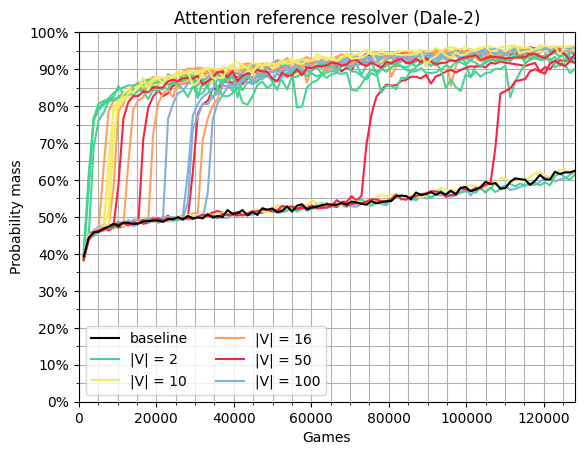
\includegraphics[width=0.3\linewidth]{figures/learning-curve_attention-predictor_dale-2_vocab-size.png}
    \label{fig:learning-curve_attention-predictor_dale-2_vocab-size}
  }
  \subfigure['Dale-5' dataset with different $|V|$ highlighted]{
    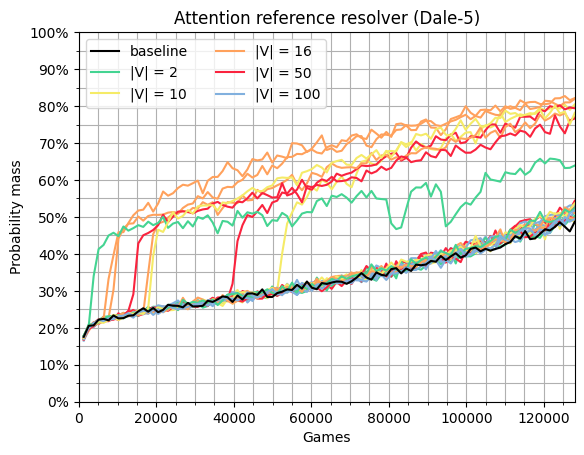
\includegraphics[width=0.3\linewidth]{figures/learning-curve_attention-predictor_dale-5_vocab-size.png}
    \label{fig:learning-curve_attention-predictor_dale-5_vocab-size}
  }
  \subfigure['CLEVR color' dataset with different $|V|$ highlighted]{
    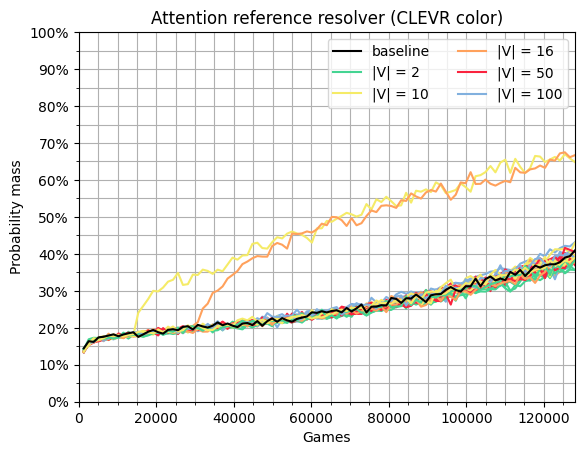
\includegraphics[width=0.3\linewidth]{figures/learning-curve_attention-predictor_colour_vocab-size.png}
    \label{fig:learning-curve_attention-predictor_colour_vocab-size}
  }
  \caption{Learning curves of all language games on each dataset. The colors correspond to different vocabulary sizes $|V|$. The baseline is marked in black.}
  \label{fig:learning-curves_attention-predictor}
\end{figure*}

% SD 2025-06-02 19:33:31 +0200: Add explanations what different versions of the same coloured curve mean.
% DK 2025-06-03 10:00:00 +0200: (done)

% SD 2025-06-02 19:38:22 +0200: To save space put the figures sides-by-side. I normally use minipage
%
% \begin{center}
%   \begin{minipage}{.5\textwidth}
%     \begin{center}
%       \includegraphics[width=0.9\textwidth]{jpg}
%       % \vspace{\textwidth}

%       Text 
%     \end{center}
%   \end{minipage}%
%   \begin{minipage}{.5\textwidth}
%    \begin{center} 
%      \includegraphics[width=0.9\textwidth]{jpg}

%      Text
%      \end{center}
%    \end{minipage}%
% \end{center}
% DK 2025-06-03 10:00:00 +0200: (done)


\begin{table}[ht]
  \footnotesize
  \centering
  \begin{tabular}{cc|c|c|c}
    \toprule
                                  &           & \multicolumn{1}{c}{\textbf{Dale-2}} & \multicolumn{1}{c}{\textbf{Dale-5}} & \multicolumn{1}{c}{\textbf{color}} \\  \cmidrule(lr){3-3}\cmidrule(lr){4-4}\cmidrule(lr){5-5}
    $n$                           & $|V|$     & \textbf{$P$ mass}                   & \textbf{$P$ mass}                   & \textbf{$P$ mass}                  \\\midrule
    \multicolumn{2}{c|}{baseline} & {62,16\%} & {49,61\%}                           & {41,68\%}                                                                \\\midrule
    {2}                           & {2}       & {92,27\%}                           & \textcolor{red}{52,15\%}            & \textcolor{red}{33,64\%}           \\
    {3}                           & {2}       & {94,52\%}                           & \textcolor{red}{51,97\%}            & \textcolor{red}{37,09\%}           \\
    {4}                           & {2}       & {89,15\%}                           & \textcolor{red}{51,98\%}            & \textcolor{red}{39,68\%}           \\
    {6}                           & {2}       & \textcolor{red}{59,68\%}            & \textcolor{red}{53,57\%}            & \textcolor{red}{38,43\%}           \\
    {2}                           & {10}      & \textbf{96,16\%}                    & {80,26\%}                           & \textcolor{red}{36,53\%}           \\
    {3}                           & {10}      & {94,9\%}                            & \textcolor{red}{53,47\%}            & \textcolor{red}{38,24\%}           \\
    {2}                           & {16}      & {95,84\%}                           & \textbf{84,03\%}                    & \textcolor{red}{39,65\%}           \\
    {4}                           & {10}      & \textbf{96,08\%}                    & \textcolor{red}{48,03\%}            & \textbf{64,31\%}                   \\
    {3}                           & {16}      & {94,59\%}                           & \textbf{81,46\%}                    & \textbf{67,88\%}                   \\
    {6}                           & {10}      & \textcolor{red}{63,46\%}            & \textbf{82,12\%}                    & \textcolor{red}{40,11\%}           \\
    {4}                           & {16}      & {94,14\%}                           & \textcolor{red}{49,81\%}            & \textcolor{red}{40,84\%}           \\
    {6}                           & {16}      & {95,86\%}                           & \textcolor{red}{50,71\%}            & \textcolor{red}{40,61\%}           \\
    {2}                           & {50}      & {93,78\%}                           & \textcolor{red}{52,24\%}            & \textcolor{red}{39,56\%}           \\
    {3}                           & {50}      & {93,88\%}                           & {79,65\%}                           & \textcolor{red}{40,36\%}           \\
    {2}                           & {100}     & {92,43\%}                           & \textcolor{red}{53,23\%}            & \textcolor{red}{37,68\%}           \\
    {4}                           & {50}      & \textbf{96,24\%}                    & \textcolor{red}{48,79\%}            & \textcolor{red}{43,61\%}           \\
    {3}                           & {100}     & {95,25\%}                           & \textcolor{red}{48,52\%}            & \textcolor{red}{42,55\%}           \\
    {6}                           & {50}      & {91,27\%}                           & \textcolor{red}{52,55\%}            & \textcolor{red}{40,21\%}           \\
    {4}                           & {100}     & {95,55\%}                           & \textcolor{red}{49,65\%}            & \textcolor{red}{42,85\%}           \\
    {6}                           & {100}     & \textcolor{red}{60,27\%}            & \textcolor{red}{46,92\%}            & \textcolor{red}{41,98\%}           \\
    \bottomrule
  \end{tabular}
  \caption{Probability masses of the attention reference resolver after 128.000 games: $n$ are different maximum message lengths and $|V|$ are different vocabulary sizes. Results in red didn't pass the baseline. The results are sorted by the product of $n$ and $|V|$ which corresponds to available space for the message. The best results are achieved with a medium-sized message space across all datasets.}
  \label{tab:results:attention-reference-resolver-game}
\end{table}

% SD 2025-06-02 19:58:12 +0200: An idea: if we multiply n * V we get the number of possible cominations, right? If we rankend the results this way they would be comperable and show the interaction between the vocabulary size and message length.
% DK 2025-06-03 10:00:00 +0200: (done)

The final probability masses after 128.000 games are summed up in Table \ref{tab:results:attention-reference-resolver-game}.
Interestingly, the baseline can already find and attend to the correct regions in many cases without the help of the sender.
The probability mass is higher than a uniform distribution ($\approx$ 4,6\%) and a random guess of an object.
It reaches 62,16\% on the 'Dale-2' dataset, 49,61\% on the 'Dale-5' dataset and 41,68\% on the 'CLEVR color' dataset.
Looking at the 'Dale-2' dataset, almost all configurations beat the baseline and achieve performances of over 90\%, the best configurations reach even 96\%.
Only three configurations stay on the level of the baseline. % SD 2025-06-02 19:53:41 +0200: Shown in red.
% DK 2025-06-03 10:50:12+0200: added to table caption
When comparing the results, mostly the message length $n$ seems to have an influence on the performance.
While configurations with $n=6$ can perform well, this is not constant.
All three configurations that don't pass the baseline are allowed to produce message with $n=6$.
$n \in \{3,4\}$ seem to help the agents the most to perform consistently well, but the difference to configurations with $n=2$ is very small.
In both cases, the target object is unambiguously identified.
The small number of experiments doesn't allow definite conclusions on the influence of the vocabulary size $|V|$, though $|V|=2$ performs slightly worse than the remaining vocabulary sizes.
A correlation between $n$ and $|V|$ is not identifiable.

On the 'Dale-5' dataset, the agents already have bigger problems to beat the baseline.
Only 8 out of 30 configuration perform better and reach probability masses around 76\% to 84\%.
However, the increase compared to the baseline is as high as on the 'Dale-2' dataset, with around 30\% points.
Smaller message lengths ($n \in \{2,3\}$) as well as a medium-sized vocabulary ($|V| \in \{10,16,50\}$) tend to help the agents more, to solve the task successfully.
As before, no correlation is visible with the few successful games.
That the agents struggle more with the 'Dale-5' dataset is not surprising.
First, the larger number of distractors makes it more difficult for the receiver to focus, as can be seen already in the baseline performances.
Additionally, the larger number of objects also influences the referring expression needed to uniquely describe the target object.
With an increasing number of distractors, the probability rises that the target object shares attributes with any distractor.
Therefore, it is more likely that the sender needs to use two or three attributes to describe the target object on the 'Dale-5' dataset compared to the 'Dale-2' dataset.
This is naturally more complex to learn for the agents. % SD 2025-06-02 20:01:28 +0200: is this really the case? In Figure 1 we have several objects and attributes but "the brown" can only be distinguished by one attribute. The goal is to always control the number of the attributes that are needed to describe the target rather than the number of attributes that are shared in the image, right? In this experiment we do not distinguish this because all are agreggated for the dataset, right? There is a difference between the complexity of the scene in terms of the attributes and the complexity of the shortest referring expresssion needed to identify the target. This is something that I still have a hard time to remember which one we are doing in this work. Can we expand on this a bit more?
% DK 2025-06-03 10:50:12+0200: (done)
Finally, since more objects are present, they are more likely clustered closer together, which can result in the identification of adjacent regions to the target regions.

The agents struggle the most on the 'CLEVR color' dataset.
In this case, only two configurations perform better than the baseline and reach a probability mass of around 64\% to 67\%.
Both utilize a medium message length of $n \in \{3,4\}$ and a medium-sized vocabulary of $|V| \in \{10,16\}$.
Interestingly, several configurations with short message lengths of $n=2$ perform worse than the baseline.
This indicates that there is communication between the agents, but it rather distracts the receiver from the target object towards the distractors.
The same point for a more difficult task when more objects are involved can be made for the 'CLEVR color' dataset.
This dataset includes even up to 10 objects present in the scene which increases the likelihood that the receiver focuses on a wrong object.

\begin{figure}[!htbp]
  \centering
  \subfigure['Dale-2']{
    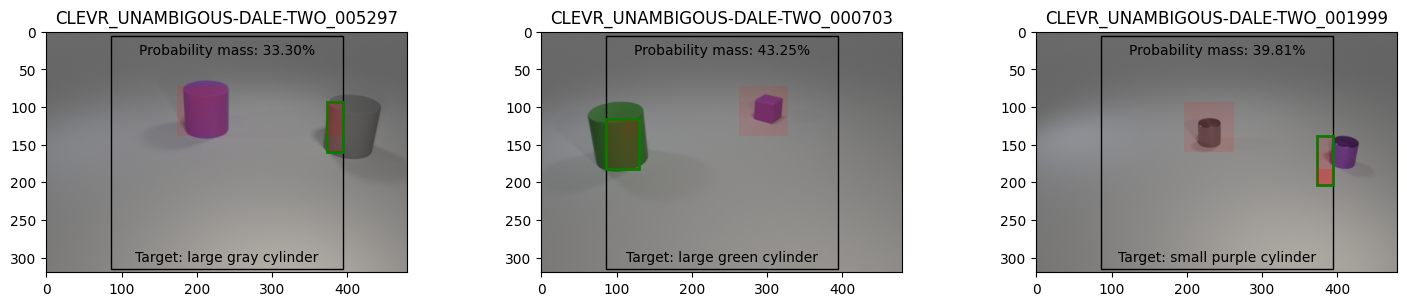
\includegraphics[width=\linewidth]{figures/visualization_games_dale-2_attention.png}
    \label{fig:visualizations_game_dale-2_attention}
  }
  \subfigure['Dale-5']{
    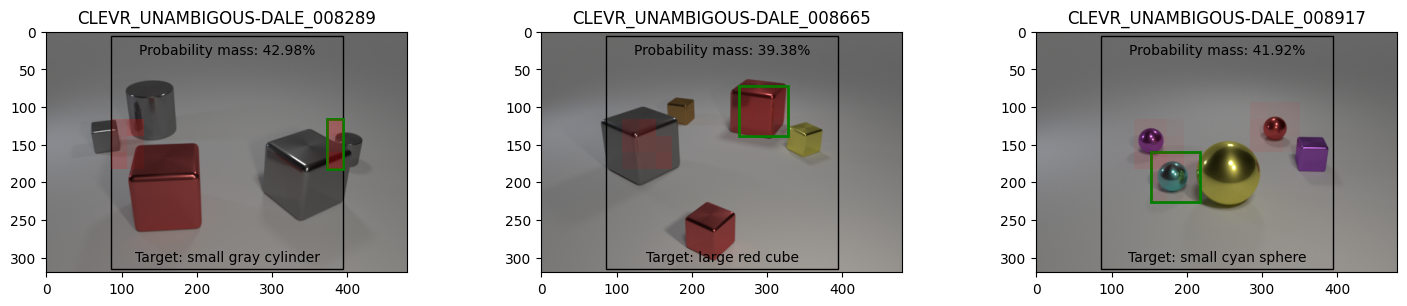
\includegraphics[width=\linewidth]{figures/visualization_games_dale-5_attention.png}
    \label{fig:visualizations_game_dale-5_attention}
  }
  \subfigure['CLEVR color']{
    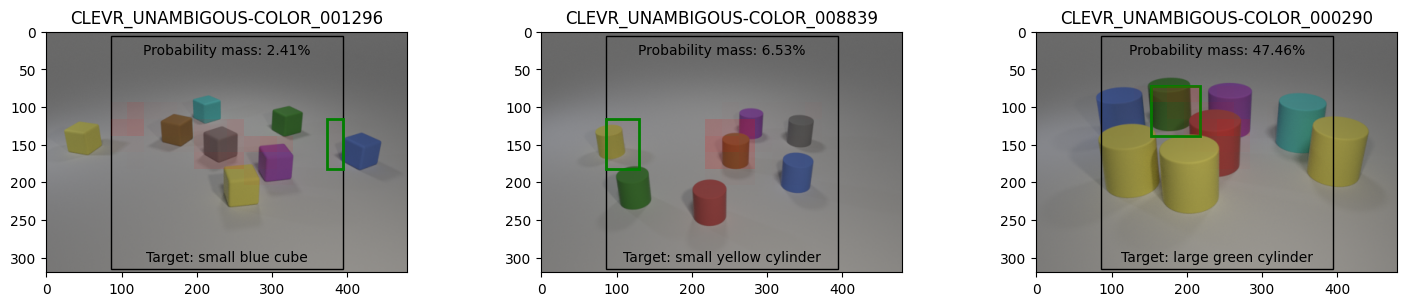
\includegraphics[width=\linewidth]{figures/visualization_games_colour_attention.png}
    \label{fig:visualizations_game_colour_attention}
  }
  \caption{Examples of the predictions in language games with successful communication with a probability mass lower than 50\% on the 'Dale' and 'CLEVR color' datasets. The black rectangle shows the cropped section the model is actually seeing after the image is preprocessed for ResNet-101. The green rectangle surrounds the target region that needs to be predicted while the red regions show the actual predictions of the model. The more intense the red, the higher is the probability that the model assigned to this region.}
  \label{fig:visualizations_game_attention}
\end{figure}

Figure \ref{fig:visualizations_game_attention} shows examples of the wrongly identified regions on each dataset.
These are predictions by the agents that are wrong even though a language emerged successfully.
Main problems seemed to be target objects not being in the actual frame of the scene that the receiver was processing.
This happens due to center cropping the image to prepare it as input for the ResNet model. % SD 2025-06-02 20:10:47 +0200: How could this happen? The scene has been trimmed, right?
% DK 2025-06-03 10:00:00 +0200: (done)
However, in several cases (as in the central image), especially for the 'Dale-5' dataset, all objects are visible, and the agents still don't attend solely on the target object.
Rather than choosing one of the distractors, the agents usually attend to both objects relatively equally.
This indicates that the receiver is uncertain which object the sender is describing.
In contrast, the share of errors of the latter type is drastically higher.
While a general pattern is difficult to identify, the receiver tends to confuse the target object with distractors that share multiple attributes with each other.
In the central and right image, the wrongly identified distractors share both \emph{size} and \emph{shape} with the target object.

\subsection{Sender and receiver with natural language referring expressions}
Two further experiments are conducted to have a closer look at the sender and receiver models.
More precisely, we evaluate how introducing explicit natural language bias into the models changes the training and ability to solve the tasks.
This is done by training both the sender and receiver models separately outside a language game context, while the architecture stays the same.
Instead of generating and respectively understanding a message of an emergent language, natural language referring expressions are used.
Here, we know that the symbols are grounded in the visual scenes and correspond to attributes of the objects.

\subsubsection{Referring expression generation (sender)}
First, instead of generating a message for the receiver, the sender is now tasked to generate natural language referring expressions.
The referring expressions for the target object are generated using the incremental GRE-algorithm \citep{Dale1995}. % , described in Section \ref{sec:background:re}.
By this, the model needs to describe the target object with respect to the distractor objects.

% \begin{figure}[ht]
%         \centering
%         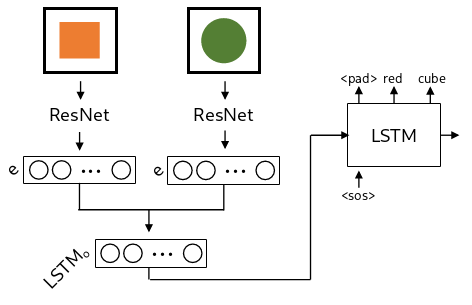
\includegraphics[width=\linewidth]{figures/arch_bb_caption_generator.png}
%         \caption{Simplified architecture of the bounding box RE generator}
%         \label{fig:bb_re_generator_architecture}
% \end{figure}

During testing, the LSTM is always forced to generate three tokens, with an embedded \texttt{<sos>} token as first input to the LSTM.
Each token in the sequence is determined greedily, by selecting the highest logit in the output of each step in the LSTM.
Training is done for 30 epochs and with a learning rate of $2\times10^{-4}$.
The loss is calculated using cross entropy.

This task can be interpreted as a classification task rather than a natural language generation task, as the model is tasked to assign specific attributes to the target object instead of producing free text with a large vocabulary.
Furthermore, the model's success is validated on accuracy, recall and precision scores.
The \textbf{overall accuracy} is a measure if the model predicted every word in the referring expression correctly.

\begin{table}[ht]
  \centering
  \begin{tabular}{c|cc}
    \toprule
                         & \textbf{Accuracy} & \textbf{F1-Score} \\\midrule
    \textbf{Dale-2}      & 99\%              & 98,57\%           \\
    \textbf{Dale-5}      & 69\%              & 89,53\%           \\
    \textbf{CLEVR color} & 93\%              & 95,17\%           \\
    \bottomrule
  \end{tabular}
  \caption{Overall accuracies (Accuracy) and F1-Scores after 30 epochs with embedding size $e=100$, $LSTM_o=500$ and $LSTM_e=30$.}
  \label{tab:results:bb-re-generator}
\end{table}

Table \ref{tab:results:bb-re-generator} shows the \emph{overall accuracy} and \emph{F1 scores} for each word.
As can be seen, the overall accuracies, in other words perfect matches of the generated referring expression depend very much on the dataset.
With the 'Dale-2' and 'CLEVR color' dataset, the model can achieve high scores of 99\% and 93\% if the samples.
In contrast, the model can only generate perfect referring expressions in 69\% of the samples of the 'Dale-5' dataset.

\begin{table*}[ht]
  \centering
  \begin{tabular}{rr|cc|c|ccc|c|c}
    \toprule
                                     &             & {small} & {large} & \textbf{size}  & {cube}  & {cylinder} & {sphere} & \textbf{shape} & {\texttt{<pad>}} \\\midrule
    \multirow{2}{*}{\textbf{Dale-2}} & {Precision} & {99,17} & {98,29} & \emph{98,73} & {99,86} & {99,71}    & {99,67}  & \emph{99,75} & {99,64}          \\
                                     & {Recall}    & {97,54} & {94,26} & \emph{95,9}  & {100}   & {99,56}    & {99,67}  & \emph{99,74} & {99,77}          \\\midrule
    \multirow{2}{*}{\textbf{Dale-5}} & {Precision} & {69,65} & {69,21} & \emph{69,43} & {98,19} & {98,32}    & {98,39}  & \emph{98,3}  & {82,22}          \\
                                     & {Recall}    & {62,11} & {66,15} & \emph{64,13} & {98,79} & {97,87}    & {98,25}  & \emph{98,3}  & {84,59}          \\\midrule
    \multirowcell{2}[0pt][r]{\textbf{CLEVR}                                                                                                                   \\\textbf{color}} & {Precision}  & {-}     & {-}     & \textbf{-}     & {100}   & {100}      & {100}    & \emph{100}   & {100}   \\
                                     & {Recall}    & {-}     & {-}     & \emph{-}     & {100}   & {100}      & {100}    & \emph{100}   & {100}            \\
    \bottomrule
  \end{tabular}
  \caption{Precision and Recall in \% for \texttt{<pad>}, size and shape tokens with $e=100$, $LSTM_o=500$ and $LSTM_e=30$. The columns \textbf{shape} and \textbf{size} show the average across all tokens of the respective attribute.}
  \label{tab:results:bb-re-generator_size-shape}
\end{table*}

\begin{table*}[ht]
  \centering
  \begin{tabular}{rr|cccccccc|c}
    \toprule
                                     &             & {blue}  & {brown} & {cyan}  & {gray}  & {green} & {purple} & {red}   & {yellow} & \textbf{color} \\\midrule
    \multirow{2}{*}{\textbf{Dale-2}} & {Precision} & {94,51} & {98,77} & {97,59} & {98,68} & {98,89} & {98,8}   & {97,47} & {100}    & \emph{98,09} \\
                                     & {Recall}    & {97,73} & {100}   & {98,78} & {97,4}  & {96,74} & {98,8}   & {100}   & {98,8}   & \emph{98,53} \\\midrule
    \multirow{2}{*}{\textbf{Dale-5}} & {Precision} & {92,12} & {93,82} & {89,13} & {89,12} & {92,63} & {91,12}  & {97,24} & {94,36}  & \emph{92,44} \\
                                     & {Recall}    & {92,12} & {89,78} & {94,91} & {94,51} & {95,71} & {92,42}  & {89,34} & {94,85}  & \emph{92,95} \\\midrule
    \multirowcell{2}[0pt][r]{\textbf{CLEVR}                                                                                                           \\\textbf{color}} & {Precision}           & {93,46} & {92,37} & {94,47} & {93,86} & {92,04} & {91,13}  & {90,07} & {94,7}   & \emph{92,76} \\
                                     & {Recall}    & {92,75} & {92}    & {95,98} & {89,92} & {94,12} & {91,13}  & {94,23} & {91,91}  & \emph{92,76} \\
    \bottomrule
  \end{tabular}
  \caption{Precision and Recall in \% for color tokens with $e=100$, $LSTM_o=500$ and $LSTM_e=30$. The column \textbf{color} shows the average across all colors.}
  \label{tab:results:bb-re-generator_color}
\end{table*}

Tables \ref{tab:results:bb-re-generator_size-shape} and \ref{tab:results:bb-re-generator_color} give a more detailed insight in the results and especially what mistakes the model is making for both the 'Dale-5' and 'CLEVR color' datasets.
The tokens are grouped by attribute and also show the metrics averaged over each of the attributes.
The metrics of the \texttt{<pad>} token indicate if the model produced the correct length of the referring expression, in other words if it was able to determine which attributes are necessary to discriminate the target object from the distractors.
For the 'CLEVR color' dataset, the scores are perfect.
This is not surprising, since all referring expressions for the 'CLEVR color' dataset consist of exactly two attributes, shape and color, and the first generated token will always be the only \texttt{<pad>} token in the referring expression (corresponding to the unspecified size).
The \texttt{<pad>} token is therefore easy to learn.
For the 'Dale-5' dataset, the model struggles more to predict the correct length of the referring expression.

The shape can be identified very well across all datasets.
The model predicts the correct shape for all samples using the 'CLEVR color' dataset, while both \emph{precision} and \emph{recall} lie around 98,3\% when using the 'Dale-5' dataset.
Even though the score is almost perfect, the slight difference might stem from the fact that all distractors have the same shape in the first case, while distractors can be different in the second case.
Consequently, the model is only exposed to one shape at a time for each sample, which might simplify its identification.

For the color attribute, the metrics drop significantly for both 'Dale-5' and 'CLEVR color' to an average of around 93\%.
Hereby, no meaningful difference can be seen across the datasets, but there are differences between the colors.
Some colors are predicted with \emph{precision} and \emph{recall} around 95\% to 96\%, while others are only around 90\%.
However, these differences are not reproducible across multiple runs and configurations.
The best and worst predicted colors vary and no conclusions can be drawn which colors are easier to predict for the model.

Finally, the size is the most difficult attribute to predict for the model.
Apart from the 'CLEVR color' dataset, where a size never needs to be predicted and also is never predicted, the metrics for the prediction of size tokens are the lowest across all tokens.
They are the only mistakes, the model makes, when exposed to the 'Dale-2' dataset and the average \emph{precision} lies around 23\% below the average of predictions of the color for the 'Dale-5' dataset, while the average \emph{recall} lies around 28,82\% below.
The reason why the \emph{precision} is higher than the \emph{recall} is the \texttt{<pad>} token, which is predicted very often instead of a token specifying the size.
In fact, the opposite relationship is visible for the \emph{precision} and \emph{recall} for said token.
The much higher absolute number of \texttt{<pad>} tokens leads to a smaller relative difference of \%-points shown in the table.
Again, no conclusion can be drawn if larger or smaller objects are easier to predict, since the results vary across runs and configurations.

In conclusion, the model successfully extracts discriminative features and produces referring expressions, though performance depends heavily on the number of distractors. Shape attributes are most easily identified, while size attributes prove most challenging.

\subsection{Referring expression resolution (receiver)}
As before, the setup of the receiver model stays the same for this experiment, but instead of interpreting the sender's message, natural language referring expressions are passed to the model.
As we know that the referring expressions are grounded in the scene, we can now compare the results to the language games, where the agents needed to learn and ground the arbitary vocabulary first.

% \begin{figure}[ht]
%         \centering
%         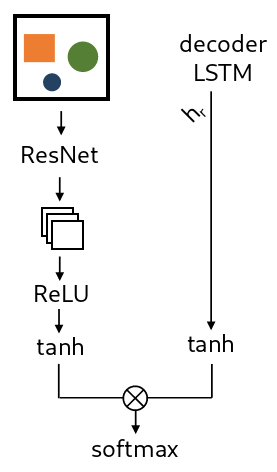
\includegraphics[width=.4\linewidth]{figures/arch_attention_predictor.png}
%         \caption{Simplified architecture of the attention predictor}
%         \label{fig:attention_predictor_architecture}
% \end{figure}

\begin{table}[ht]
  \centering
  \begin{tabular}{c|c}
    \toprule
                         & \textbf{Probability mass} \\\midrule
    \textbf{Dale-2}      & {95,16\%}                 \\
    \textbf{Dale-5}      & {92,19\%}                 \\
    \textbf{CLEVR color} & {95,33\%}                 \\
    \bottomrule
  \end{tabular}
  \caption{Probability masses of the model after 20 epochs with $LSTM_e=15$ and $LSTM_o=1500$.}
  \label{tab:results:attention-reference-resolver}
\end{table}

The results are shown in Table \ref{tab:results:attention-reference-resolver}.
Across all datasets, the model is able focus on the correct region in the image with high precision of over 90\%.
Interestingly, a different pattern emerges when comparing the results to the language games.
While both agents and the single model achieved the best scores with the 'Dale-2' dataset, the single model can achieve similar results on the 'CLEVR color' dataset.
On the 'Dale-5' dataset, the performance is slightly worse.
In contrast, the agents achieved better results on the 'Dale-5' dataset, and struggled mostly with learning and grounding colors.

\section{Discussion and Conclusion}
We demonstrate a method for conducting focused experiments on artificial data through which we gain valuable insights what particular models are capable of learning from data and their dependence on the structure and representations in the data in the context of linguistic coordination and learning over a visual scene.
This knowledge can be transferred to the design of larger systems that are trained on real data to gain insights about learning architectures, representations of features and datasets.
They can also be used as a diagnostic probes for systems trained on real data.

Our language games revealed that agents can successfully develop communication protocols, achieving substantial performance gains over baselines.
However, emergent communication faces constraints: medium-sized vocabularies and message lengths proved most effective.
Scene complexity significantly impacts learning, with simpler scenes enabling near-perfect communication while complex scenes challenged most configurations.

The natural language experiments provided crucial insights into these limitations.
When generating referring expressions, models achieved high accuracy on simple scenes but struggled with complex discriminations.
Critically, the \emph{size} attributes proved most difficult to learn across all tasks, followed by the \emph{color}, while the \emph{shape} was consistently well-identified.
This indicates that humans and artificial neural networks have quite different learning biases that facilitate learning for humans (e.g. pragmatic referring described in the Dale-Reiter algorithm) is difficult to learn for systems.
The experiments demonstrate that once we add such learning biases (e.g. modelling focused attention) learning becomes more successful.
Overall, the results indicate that to be successful, learning language and vision models needs to go beyond mere observation of pixels and words.

Future work should investigate the linguistic properties of the emergent languages to better understand how agents encode visual attributes in their communicative protocols.
Detailed analysis of message patterns could reveal whether emergent languages develop similar structures seen in natural languages.

\bibliographystyle{acl_natbib}
\bibliography{custom}

\appendix

\section{Technical details of the language games}
\label{app:technical-details-language-games}
The sender extracts the features of each bounding box using ResNet-101 and projects them to an image embedding dimension $e_r=100$ with a linear layer.
All encoded bounding boxes are concatenated and again compressed to the decoder output dimension $h_s=500$ using another linear layer.
This representation of all objects serves as the initial hidden state of an LSTM, which generates the referring expression.
Tokens used in the LSTM are embedded with embedding dimension $LSTM_{s,e}=100$.
During training, teacher forcing is applied by using embeddings of the ground truth tokens as the input sequence for the LSTM, instead of the output of the LSTM.

The receiver decodes the sender's message using an LSTM with a hidden size $h_r=500$ and token embedding dimension of $LSTM_{r,e}=100$.
The image is encoded using a combination of ResNet-101 and several convolutional layers described in Section \ref{sec:image-processing}.
Both encodings are passed through a $tanh$ non-linearity, and the results are combined using a dot product.
The resulting vector is passed through a $softmax$ function to produce a probability distribution over the 14$\times$14 regions of the image.

The experiments are conducted with the following hyperparameters: a learning rate of $2\times10^{-4}$, a temperature for the Gumbel-Softmax relaxation of 1 and \emph{Adam} \citep{Kingma2015} as optimizer.

The source code for all experiments is available at \href{https://github.com/DominikKuenkele/MLT\_Master-Thesis}{github.com/DominikKuenkele/MLT\_Master-Thesis}.

\end{document}
